% format de la feuille
% taille police globale (pas les titres)
% recto (oneside) ou recto-verso (twoside)
% fleqn pour numéroter les équations à droite
% classe : article, book, report
\documentclass[a4paper,fleqn,12pt]{report}

% ---------------------------------------------------------------------------------------------------------
% LANGUES ET POLICE
\usepackage[frenchb, english]{babel} % langue principale : français
\usepackage[utf8]{inputenc} % encodage 
\usepackage[T1]{fontenc} % accents
\usepackage{lmodern} % police vectorielle
\usepackage{ulem} % souligner
\usepackage[usenames,dvipsnames,svgnames,table]{xcolor} % pour écrire en couleur 

% ---------------------------------------------------------------------------------------------------------
% CARACTERES SPECIAUX + MATH
\usepackage{csquotes} % beaux guillemets \enquote{texte}
\usepackage{amssymb} % symboles mathématiques
\usepackage{listings} % inclure du joli code
\usepackage{listingsutf8}
\usepackage{amsmath} % formules mathématiques, flèches etc
\usepackage{amsfonts} % fraktur etc. 
\newcolumntype{M}[1]{>{\raggedright}m{#1}}
\lstset{
  language=Java,
  basicstyle=\ttfamily,
  columns=fullflexible,
  frame=single,
  breaklines=true,
  postbreak=\mbox{\space},
  numbers=left,
  numberstyle=\tiny,
  showspaces=false,
  showtabs=false,
  showstringspaces=false,
  breakatwhitespace=true,
  commentstyle=\color{MidnightBlue},
  keywordstyle=\color{blue},
  stringstyle=\color{ForestGreen},
  moredelim=[il][\textcolor{gray}]{\$\$},
  moredelim=[is][\textcolor{gray}]{\%\%}{\%\%},
  literate=%
         {é}{{\'e}}1
         {è}{{\`e}}1
         {ú}{{\'u}}1   
         {ù}{{\`u}}1
         {Á}{{\'A}}1
         {É}{{\'E}}1
         {ê}{{\^e}}1
         {Ê}{{\^E}}1
}
\lstdefinelanguage{json}{
    basicstyle=\normalfont\ttfamily,
    numbers=left,
    numberstyle=\scriptsize,
    stepnumber=1,
    numbersep=8pt,
    showstringspaces=false,
    breaklines=true,
    frame=lines,
    backgroundcolor=\color{white},
    literate=
     *{0}{{{\color{MidnightBlue}0}}}{1}
      {1}{{{\color{MidnightBlue}1}}}{1}
      {2}{{{\color{MidnightBlue}2}}}{1}
      {3}{{{\color{MidnightBlue}3}}}{1}
      {4}{{{\color{MidnightBlue}4}}}{1}
      {5}{{{\color{MidnightBlue}5}}}{1}
      {6}{{{\color{MidnightBlue}6}}}{1}
      {7}{{{\color{MidnightBlue}7}}}{1}
      {8}{{{\color{MidnightBlue}8}}}{1}
      {9}{{{\color{MidnightBlue}9}}}{1}
      {:}{{{\color{black}{:}}}}{1}
      {,}{{{\color{black}{,}}}}{1}
      {\{}{{{\color{ForestGreen}{\{}}}}{1}
      {\}}{{{\color{ForestGreen}{\}}}}}{1}
      {[}{{{\color{ForestGreen}{[}}}}{1}
      {]}{{{\color{ForestGreen}{]}}}}{1},
      literate=%
         {é}{{\'e}}1
         {è}{{\`e}}1
         {ú}{{\'u}}1
         {ù}{{\`u}}1
         {Á}{{\'A}}1
         {É}{{\'E}}1
         {ê}{{\^e}}1
         {Ê}{{\^E}}1
}
% ---------------------------------------------------------------------------------------------------------
% LISTES
\usepackage{enumitem} % customiser les listes
%\frenchbsetup{StandardLists=true} % éviter les conflits avec enumitem
\setlist[itemize]{noitemsep, topsep=0pt}
\setlist[enumerate]{noitemsep, topsep=0pt}
\setlist[description]{noitemsep, topsep=0pt}
% ---------------------------------------------------------------------------------------------------------
% TABLEAUX ET FIGURES
\usepackage[sc,footnotesize]{caption} % légendes des tableaux et figures
\usepackage{subfig} % plusieurs figures côte à côte (subfloat)
\usepackage{longtable} % autoriser que les longs tableaux débordent sur plusieurs pages
\usepackage{multicol} % fusionner les colonnes dans un tableau
\usepackage{multirow} % fusionner les lignes dans un tableau
\usepackage{caption} % pour les légendes
\usepackage{slashbox} % pour les Tableaux comparatifs
\usepackage{graphicx} % insérer image
\usepackage{rotating}
\usepackage{epstopdf}
\usepackage{wrapfig}

\usepackage{fancybox}
\graphicspath{{figures/}} % dossier dans lequel sont les images
%\usepackage{tikz} 	% outil de modélisation de formes

% ---------------------------------------------------------------------------------------------------------
% MISE EN PAGE 
\usepackage{lscape}
\usepackage{setspace}
\usepackage{verbatim}

\raggedbottom

% - Marges
\usepackage[top=2cm, bottom=2cm, left=2cm, right=2cm ]{geometry} % marges

% - Page style
\pagestyle{headings}

\DeclareUnicodeCharacter{00A0}{ }
% - Alinéas et espacements entre paragraphes
\usepackage{parskip}
\parskip = 10pt % espace
\parindent = 0pt % alinéa

% - Style des sections
\usepackage{titlesec}
\titleformat*{\section}{\Large\scshape}
\titleformat*{\subsection}{\large\scshape}
\titleformat*{\subsubsection}{\scshape}

\pagestyle{plain}
%---------------------------------------------------------------------------------------------------------
\selectlanguage{frenchb}
\author{Gilles Bodart}
\date{\today}
\title{Archipelago}
\begin{document}
\thispagestyle{empty}

\begin{center}
\textsc{Universit\'e de Namur}\\
Facult\'e d'informatique\\
Ann\'ee acad\'emique 2017--2018
\end{center}
\vspace{1.3cm}
\hspace{1.4cm}
\begin{center}
\fbox{
\begin{minipage}[c][5.4cm]{11cm}
\large
\begin{spacing}{1.2}
\begin{center}
\textbf{Archipelago : Un framework de peristence pour bases de données orientées graph.}
\\
\vspace{0.5cm}
Gilles Bodart
\end{center}
\end{spacing}
\end{minipage}
}
\end{center}


\vspace{0.5cm}
\begin{figure}[!h]
\centering
\includegraphics[width=.4\textwidth]{figures/unamur.pdf}
\end{figure}

\normalsize


\vspace{0.5cm}
\begin{table}[!h]
\centering
  \begin{tabular}{ r l }
    Promoteur~: &  \rule{4cm}{0.1mm} {\small (Signature pour approbation du d\'ep\^ot - REE art. 40)}\\
    ~\underline& CLEVE Anthony \\\\
    Co-promoteur~: & LAMBIOTTE Renaud  \\
  \end{tabular}
\end{table}

\vspace{0.5cm}
\begin{center}
M\'emoire pr\'esent\'e en vue de l'obtention du grade de\\
Master en Sciences Informatiques.
\end{center}
\tableofcontents
\newpage


\chapter*{Introduction}

De nos jours, les unités de stockages sont de plus en plus accessible au grand public, les différentes entreprises impliquées dans le développement des systèmes de gestion de base de données l'ont bien compris. Depuis plusieurs années, L'hégémonie des bases de données relationnelles se fait de moins en moins écrasante, le solutions alternatives du NoSql séduisent jours après jours de grandes entreprises. 

La grande force des SGBDR provient des fondement théorique mis en place en 1970 par Edgar Frank Codd, IBM défini le langage "Structured Query Language" (SQL) pour utiliser ce système. Cette normalisation de la représentation de l'information génère un sentiment de sûreté pour les architectes de logiciels.

A contrario, le mouvement NoSql pour "Not Only SQL" ne se base pas sur un fondement théorique commun. Que ce soit la théorie des graphs, les systèmes de hash key/value avec partitions, ... chaque système choisit ce sur quoi il va se baser. Mais si il existait une sorte de contrat liant les SGBD NoSql entre eux afin d'assurer une cohérence d'utilisation, ce mémoire va se concentrer sur les implémentations de la théorie des graph, en essayant de mettre en place un système de comparaison, nous allons tenter de spécifier certains objectifs commun et développer un framework Java permettant d'utiliser de manière agnostique l'une ou l'autre base de donnée.
 
\part{État de l'art}

\chapter{L'évolution du NoSql}
\label{NoSqlEvol}

Un SGBD est par définition un ensemble de procédés permettant d'organiser et de stocker des informations (potentiellement de gros volumes). Si stocker et retrouver l'information est un des plus grand challenge d'un SGBD, une communauté de développeur, pensent que ces système devraient pouvoir offrir d'autres fonctionnalités. 

A partir des années 1980, le modèle relationnelle supplante les autres formes de structures de donnée.

Les évolutions logicielles suivant naturellement les évolutions matérielles, la généralisation des interconnexion des réseaux, l'augmentation de la bande passante, la diminution du cout des machines, la miniaturisation des espaces de stockage, ... de nouvelles opportunités sont arrivé au XXI\up{e} siècle.

Les entreprises comme Google, Amazon, Facebook, Twitter, ... sont tour à tour arrivés aux limites du modèle Relationnel. Que ce soit a cause de volumes astronomiques (plus de 100 pétaoctets ) ou du nombre de requêtes par secondes, il fallut développer une nouvelle façon de gérer les données.

Le NoSql découle de ce genre de problèmes, ces modèles arrivent avec des approche optimisée pour des secteurs spécifiques. \\
Comme ces modèles représentent ce qui n'est pas Relationnel, par soucis de classification, nous allons distinguer 4 usages principaux :

\begin{itemize}
\item Performances : L'objectif du SGBD sera d'augmenter au maximum les performances de la manipulation des données. 
\item Structures simples : Pour s'affranchir de la rigidité du modèle relationnel, la structure sera généralement simplifiée, en utilisant une représentation plus souple comme le JSON par exemple.
\item Structures spécifiques : Certain moteur NoSql sont liés a des besoins spécifiques, la structure de représentation de donnée sera dès lors focalisée sur un cas d'utilisation.
\item Volumétries : Un des principal aspect important des SGBD NoSql est leur capacité de gérer la montée en charge de données. La distribution des traitements au travers de plusieurs clusters est un facteur très important dans la plupart des applications BigData.
\end{itemize} 

Et nous allons aussi distinguer 4 grandes familles de représentation de Schéma de données :

\begin{itemize}
\item Document : L'utilisation de format spécifiques tels que le très rependu JSON permet de stocker les données sur base de fichier.
\item Clé / Valeur : Le système le plus simple, il manipule des paires de clé/valeurs, ou accède à un élément en fonction d'une table de hachage.
\item Colonne : Inspiré de Google BigTable, la structure ressemble à la table relationnelle. On peut la comparer à une table de hachage qui va référencer une ou plusieurs colonnes.
\item Graph : La famille Graph se distingue du fait que les entités ne sont pas considéré comme des entités indépendante, mais que la relation être ces objets est tout aussi important que le contenu.
\end{itemize} 

Les implémentations de bases de données de types graph sont de plus en plus nombreuses, les relations entre les éléments permettent de parcourir le graph de manière très performante les rendent de plus en plus intéressante pour les entreprises possédant des millions de données. L'utilisation de ce genre de SGBD est dès lors tout a fait recommandé pour des entreprises intéressé entre les relations de ces donnés tels que des profils sociaux, des liens de cause a effet, des liens géographiques et bien d'autre.

\section*{Pourquoi utiliser une BDOG plutôt qu'une BD relationnelle comme Oracle ou MySql ?}

L'utilisation des SGBD relationnelle pour tout type de problème est révolue. Grâce à l'apparition de SGBD NoSQL spécifique permet dès à présent une approche plus personnalisée. En effet, comme tout système, le relationnelle a ses limites, l'approche actuelle des entreprises est plus orienté "Big Data", elles veulent tout stocker afin d'avoir le plus d'informations possible, or du fait que le relationnelle cadenasse les données dans une table préalablement définie, on se doit de tronquer l'information ou alors, mettre a jour le schéma de définition des tables. Dans une BDOG tel que Neo4J, nous pouvons ajouter toutes les informations que nous voulons sans condition préalable, cette approche oriente plus un contrôle de l'intégrité des donnée aux applications.

Si l'objectif de l'applicatif est de représenter un système récursif comme une arborescence de fichier, de la généalogie, ... le modèle relationnelle se basera sur une table faisant référence à elle même, l'utilisateur devra donc réaliser une jointure par profondeur, si l'arborescence descend jusqu'à 15 niveau, cela peut devenir problématique. L'approche BDOG permet de parcourir une arborescence sans pour autant charger l'ensemble des nœuds ayant le même label, plus besoins de projection ensembliste pour pouvoir continuer le chemin.

En relationnel, il existe de nombreux moyen d'historiser les données, cependant, lorsque le schéma comprend des relations cycliques, cette opération devient plus complexe. L'utilisation d'un BDOG rend ça plus simple, il suffit de créer un nouveau noeud avec les anciennes données, lier ce noeud avec une relation historique en y spécifiant la date de mise à jour et ensuite changer les valeur du noeud référencé par le cycle. Ce procédé peut être mis au point dans n'importe quelle représentations et ne nécessite aucune refonte globale du modèle de donnée.

\section*{On parle de Base de donnée orientée graph mais quelle est la différence entre une relation entre deux noeud et une relation entre deux table ?}
Les relations entre deux tables se font à l'aide de clé étrangère définie lors de la création du schéma de données elles apporte de l'information supplémentaire en permettant de réaliser des jointure entre plusieurs tables. 

La relation dans les BDOG est une information à part entière, elle peut posséder autant de donnée que le noeud lui même, la force de ce genre de système est de pouvoir lier deux noeud distinct par n'importe quelle relation et ce à tout moment. 

\chapter{Backgroud technique}
\section{Neo4J}

\subsection{Description}

Créé par Neo Technologie, une sociétée suédo-américaine, elle est actuellement (selon db-engines.com) la base de donnée orienté graph la plus utilisée dans le monde. Développé en java sous licence GPL V3, AGPL ou licence commerciale, Neo4J représente les données sous formes de "Noeuds" et de "Relations", chacun de ces éléments peuvent contenir une ou plusieurs propriétés. Les propriétés sont des couples clés/valeurs de type simple, comme des chaines de caractères ou des valeurs numériques, des coordonnées spatiales, ... 

Une des particularité de Neo4J est l'absence de structure définie, un noeud peut être labellisé afin de permettre de travailler sur un ensemble d'éléments, mais il n'y aura aucune contrainte sur les propriétés du noeud. Cette particularité rend ce SGBD bien adapté pour les modèles évoluant fréquemment.

\subsection{Langage de requête}

Le langage propre à Neo4J se nomme "Cypher"\label{Cypher}, il a pour but de réaliser plus simplement que SQL les opérations de parcours ou d'analyse de proximité.

\begin{lstlisting}[language=java, frame=single]
CREATE (mamours:Person {name:"Mamours"})
CREATE (mamyco:Person {name:"Mamyco"})
CREATE (gilles:Person {name:"Gilles"})
CREATE (marie:Person {name:"Marie"})
CREATE (bebe:Person {name:"Enfant"})
CREATE (mamours)-[:PARENT_OF]->(gilles)
CREATE (mamyco)-[:PARENT_OF]->(marie)
CREATE (marie)-[:PARENT_OF]->(bebe)
CREATE (gilles)-[:PARENT_OF]->(bebe)
\end{lstlisting}

Ces requêtes vont créer 5 noeud et 4 relations PARENT\_OF, nous pouvons aisément comprendre que "Mamyco" est parente de "Marie"

\begin{lstlisting}[language=java, frame=single]
MATCH (p:Person)-[:PARENT_OF]->(c:Person) 
RETURN DISTINCT (p)
	
\end{lstlisting}

Cette query va retourner tout les nœuds distinct qui ont une relation :PARENT\_OF avec un autre noeud.

\begin{lstlisting}[language=java, frame=single]
MATCH (gp:Person)-[:PARENT_OF*2]->(c:Person) 
RETURN DISTINCT (gp)
	
\end{lstlisting}

Celle-ci quant à elle va retourner toutes les personnes qui sont parent de parent et donc grand parents. 

ces deux exemples peuvent montrer la force de l'utilisation d'un SGBD de type graph pour représenter un ensemble hierarchique de données par rapport au SGBD relationnelles qui nécessiterai une double jointure sur la Table "Person".

\subsection{Communication}

Neo4J peut être utilisé sous plusieurs formes. 

La première option est une solution embarquée, ce choix peut être très intéressant en alternatif au très célèbre SQLite relationnel.

La deuxième, pour toute application distribuée, est une solution autonome pouvant tourner comme un service sur tout type de plateforme. Le protocol "Bolt", développé par "Néo Technologie" est grandement conseillé pour communiquer avec ces serveurs distants. 

Son utilisation est simple grâce à l'utilisation de la libraire native à Néo4J pour java (neo4j-java-drive) ou avec l'utilisation de l'API Rest déployée en même temps que le SGBD.

\section{OrientDB}

\subsection{Description}

OrientDB est un SGBD initialement développé en C++(Orient ODBMS) ensuite repris en 2010 en Java par Luca Garulli dans une version multi-modèle sous licence Apache 2.0, GPL et AGPL. actuellement 3ème mondial (selon db-engines.com) il offre de nombreuses fonctionnalités intéressante. 

OrientDB est base de donnée associant Document et Graph. Elle combine la rapidité et la flexibilité du type document ainsi que les fonctionnalités de relations des bases de données graph. 

Ce SGBD est composé de trois grands éléments 

\begin{itemize}
\item Document \& Vertex : Source de contenu, ces élements peuvent être considéré comme des container de données, on peut le comparer avec la ligne d'une base de données relationnelle.
\item Links \& Edge : Une arrête orientés reliant deux éléments non nécessairement distinct.
\item Property : Typée ou embarquée dans un document JSON, ceci va représenter le contenu de l'information. Ces propriétés sont bien entendu primordiales pour ordonner, rechercher, ...
\end{itemize}

Chaque Document ou Vertex appartient à une "Class", celle-ci peut être strictement définie ou plus laxiste. Comme dans la programmation orientée objet, OrientDB offre le principe de polymorphisme avec un système d'héritage entre les classes. 

OrientDB vient dans sa version community avec un système de clustering permettant à l'utilisateur de correctement gérer les montées en charges. chaque document est identifié avec une partie désignant le cluster dans lequel l'information est stockée et une autre partie désignant sa position dans ce dernier (exemple @rid: 10:12). Chaque classe peut être associée a un ou plusieur cluster, permettant d'optimiser les accès dans des ensembles  plus petits.


\subsection{Langage de requête}

OrientDB utilise une sorte de SQL avancée pour interpréter les requêtes. On peut de plus utiliser le langage Gremlin.

Voici quelques exemples d'utilisation du SQL avancé dans OrientDB.

\begin{lstlisting}[language=SQL]
CREATE CLASS Person EXTENDS V
CREATE CLASS Company EXTENDS V
CREATE CLASS WorkAt EXTENDS E
CREATE PROPERTY Person.firstname string
CREATE PROPERTY Person.lastname string
CREATE PROPERTY Company.name string
INSERT INTO Person(firstname, lastname) VALUES ("Gilles","Bodart"),("Marie","Van Cutsem")
	ou
INSERT INTO Company set name = "ACME"

\end{lstlisting}

Cet ensemble de requête ressemblant au langage SQL permet de créer deux vertex, Person et Company , un Edge WorkAt et leur associe certaine propriétés. Les deux types d'insert différent permettent comme en SQL d'ajouter un noeud.  

\begin{lstlisting}[language=SQL]
SELECT FROM V
\end{lstlisting}
\begin{center}
	\begin{tabular}{|c|c|c|c|c|c|}
   		\hline
  		\multicolumn{3}{|c|}{Metadata} & \multicolumn{3}{c|}{Properties} \\
   		\hline
   		@rid & @version & @class & firstname & lastname & name \\
   		\hline
   		10:0 & 1 & Person & Marie & Van Cutsem &  \\
   		10:1 & 1 & Person & Gilles & Bodart &  \\
   		11:0 & 1 & Company &  &  & ACME \\
   		\hline
	\end{tabular}
\end{center}

Nous pouvons observer qu'OrientDB se charge de qualifier les document de plusieurs métadata en leur octroyant par exemple un identifiant unique (\no cluster:position), un numéro de version pour permettre une gestion de transaction "full optimistic"\footnote{On laisse l'utilisateur continuer sa transaction et le refus se fera lors du commit si il y a eu une modification concurrente du même document} et le \@class représente la structure du document.

\begin{lstlisting}[language=SQL]
CREATE Edge WorkAt from 10:1 to 11:0
\end{lstlisting}

Cette petite requête va lier le document ayant l'id 10:1 au document dont l'id est 11:0 par une relation WorkAt. Nous pouvons traduire en français que Marie Van Cutsem travaille chez ACME.


\subsection{Communication}

OrientDB embarque une API Rest complète, toute actions pouvant être faite sur les interfaces web et consoles peuvent être reproduites au travers de cette API. 


\chapter{Solutions existantes}


\section{Les librairies} 

\subsection{Hibernate}

Hibernate, soutenu et développé par JBoss, à mis au point un système de relation entre le code Java et le SGBD Néo4J, en réutilisant les mêmes annotations de relations que celles employées pour les bases de données relationnelles, à savoir :

\begin{itemize}
\item @OneToOne : Relation 1-1
\item @ManyToOne : Relation n-1
\item @OneToMany : Relation 1-n
\item @ManyToMany : Relation n-n
\end{itemize}

Bien qu'à l'heure actuelle, aucune intégration avec OrientDB, un ticket est ouvert (OGM-855) depuis 2 ans auprès d'Hibernate.

\subsection{Spring Data}

Spring data à nouveau possède un module de communication avec le SGBD Néo4J, il intègre au célèbre Framework Spring les fonctionnalités de Néo4J-OGM\footnote{Object Graph Mapper}, permettant de qualifier une classe avec certaines annotations facilitant la séréalisation et le déséréalisation vers la représentation graphique.

Exemple : 

\begin{lstlisting}
@NodeEntity(label="Film")
public class Movie {

   @GraphId Long id;

   @Property(name="title")
   private String name;
}

@NodeEntity
public class Actor extends DomainObject {

   @GraphId
   private Long id;

   @Property(name="name")
   private String fullName;

   @Relationship(type="ACTED_IN", direction=Relationship.OUTGOING)
   private List<Role> filmography;

}

@RelationshipEntity(type="ACTED_IN")
public class Role {
    @GraphId   
    private Long relationshipId;
    @Property  
    private String title;
    @StartNode 
    private Actor actor;
    @EndNode   
    private Movie movie;
}
\end{lstlisting}

\subsection{Librairie Neo4J}

Une librairie java développée par NeoTechnologie existe, elle permet de travailler aisément avec une base de donnée Neo4J embarquée ou à distance. Elle est en constante évolution et se trouve sur une plateforme open source. 

Exemple de communication avec la librairie Neo4J le protocol "Bolt":

\begin{lstlisting}[language=java]
Driver driver = GraphDatabase.driver("bolt://localhost:7687", AuthTokens.basic("matrix", "neo"));
Session session = driver.session();
session.run("CREATE (a:Person {firstName:{name},lastName:{lastName}})", parameters("firstName","Gilles","lastName","Bodart"));
session.close();
driver.close();

\end{lstlisting}

Bien que cette libraire soit efficace, elle ne peut être utilisée avec un autre SGBD. 

\subsection{Librairie OrientDB}

La librairie OrientDB pour java est composée de trois éléments:

\begin{itemize}
\item Graph API
\item Document API
\item Object API
\end{itemize}

La graph API d'OrientDB couvre 80\% des uses cases classique d'un utilisateur, elle supporte tout les modèles de représentations comme un unique multi-modele de donnée. Elle travaille sur des "Vertex" et des "Edges", respectivement nœud et relations et est compatible avec le standard TinkerPop

La document API elle permet de couvrir les 20\% restants, elle est plus simple d'utilisation mais n'offre une utilisation plus atomique, les relations ne peuvent par exemple qu'être unidirectionnelles tandis que la bidirectionnalité est offerte dans l'API précédent. Un document est un élément unique, pour gérer les relations entre les différents nœuds de notre modèle, il faudra gérer manuellement chaque connexion.

La dernière librairie se focalise sur les objets java, elle n'a plus été améliorée depuis la version 1.5 d'OrientDB\footnote{À l'heure de l'écriture de ce mémoire, nous sommes à la version 2.2 et la version 3 à bientôt fini sa phase de "bêta test"}

\section{Les frameworks}

\subsection{Apache TinkerPop}

Apache TinkerPop est Framework open source d'utilisation de graph, il regroupe un grand ensemble de fonctionnalités et d'algorithmes. Son écosystème est de plus en plus agrémenté de librairies externes développées par de tierces personnes.

Il se considère lui-même comme étant complexe d'utilisation pour les nouveaux développeurs car il nécessite l'utilisation d'un environnement qui leur est propre, la "Gremlin-console".

Les développeurs de ce framework on mit au point un langage de travail sur les graphs appelé "Gremlin". Le langage dont nous avons parlé en section \ref{Cypher} s'est grandement inspirer de ce dernier.

Exemple d'utilisation 

\begin{lstlisting}
gremlin> g.V() /* récupère tout les noeuds du graph */
==>v[1]
==>v[2]
==>v[3]
==>v[4]
==>v[5]
==>v[6]
gremlin> g.V(1) /* récupère le noeud d'Id 1 du graph*/
==>v[1]
gremlin> g.V(1).values('name') /* récupère le noeud d'Id 1 du graph et renvoie sa propriété 'name' */
==>marko
gremlin> g.V(1).outE('knows') /* récupère les relations 'knows' partant du noeud d'Id 1 */
==>e[7][1-knows->2]
==>e[8][1-knows->4]
gremlin> g.V(1).outE('knows').inV().values('name') /* retourne le nom des personnes que le noeud 1 connait */
==>vadas
==>josh
gremlin> g.V(1).out('knows').values('name') /* même résultat */
==>vadas
==>josh
gremlin> g.V(1).out('knows').has('age', gt(30)).values('name') /* retourne le nom des personnes plus vielle que 30 ans que le noeud 1 connait */
==>josh
\end{lstlisting}

Comme expliqué plus haut, le langage doit être exécuté dans un invite de commande ou dans un serveur Gremlin, nous sommes dès lors contraint d'installer et de configurer ce dernier pour pointer vers l'un ou l'autre SGBD.



\part{Contribution}
\chapter{Application possibles des BDOG}

\section{L'exemple parfait}

Pour la suite de ce mémoire, il est primordiale d'avoir un exemple concret de modèle habituellement persisté avec un modèle relationnelle mais qui serait sans le moindre problème transposable dans une BDOG.

\subsection*{L'école}

Imaginons la représentation d'une école composée d'élèves, de professeurs, de classes, de salles techniques, de travailleurs, ... dont   le diagramme de classes se trouve en Annexe (\ref{fig:SchoolDiagram}).

Les liens entre les différents objets peuvent être fortement nombreux, nous pouvons imaginer que les étudiants sont amis, membres de famille, ennemis, amoureux, ... de même que pour les professeurs, ils peuvent avoir les mêmes relations que les étudiants mais de plus peuvent être assigné a des cours, a des classes, ... toutes ces liaisons peuvent être fortement compliquées à représenter sur une base de donnée relationnelles. L'utilisation d'une BDOG semble être tout à fait adéquate. Durant la suite de ce mémoire, nous utiliserons donc ce modèle.

\section{Critères de comparaisons}

Dans un premier temps, il est primordiale de mettre en place une liste de critères permettant de faciliter le choix de la BDOG.

\section{Comparaison des plus grandes BDOG} 
\begin{center}

\begin{tabular}[c]{|l|M{5cm}|M{5cm}|}
\hline
\backslashbox {Critère}{BDOG} & Neo4J & OrientDB  \tabularnewline
\hline
Schema de donnée strict & X & \checkmark  \tabularnewline
\hline
Format de donnée & JSON & JSON \tabularnewline
\hline
Principe d'héritage & X & \checkmark \tabularnewline
\hline
Clusturing & Configurable & Natif \tabularnewline
\hline
Communication & BOLT (protocole propriétaire) & REST (via HTTP) \tabularnewline
\hline
Évolutivité & L'absence de schéma strict entraîne une grande liberté dans la création et la modification des nœuds & Les classes doivent préalablement configurées sur le serveur \tabularnewline \hline
Rapidité\footnotemark & 7m 10s & 4m 31s \tabularnewline \hline
Modèle de représentation & Uniquement graph & multimodèle \tabularnewline \hline

\end{tabular}
\end{center}
\footnotetext{10 000 requêtes sur le même graph de donnée avec la même requête au travers d'un appel Java}
Une idée d'arbre de décision devrait, à la fin de cette section, permettre à un utilisateur muni de ses besoins, de choisir la BDOG la plus adaptée à son projet. 

\section{Piste de normalisation}

Comme nous l'avons présenter dans le point \ref{NoSqlEvol} nous nous apercevons que le problème principal du NoSql est le manque de standard d'utilisation de ces SGBD, pour ce faire, nous allons tenter de lister un des objectifs de normalisations.

\begin{itemize}
\item Utilisation d'un langage unique
\item Système de transaction 
\item Opération de base de persistances CRUD
\item Possibilité de créer des méthodes stockée 
\item Contrôle sur les propriétés.
\end{itemize}

La suite de ce mémoire portant sur le développement d'un framework java, tentera d'offrir ces objectifs de manière abstraite aux développeurs.

\chapter{Le framework}
\section{Utilisation}

Ce framework à été basé sur l'utilisation d'annotations, à l'heure actuelle, il permet d'effectuer deux opérations:

\subsection{La persistance}

La persistance est l'élément primordiale de ce framework, afin de ne pas avoir de lien avec une BDOG propre, nous nous sommes basé sur le modèle orienté objet. La persistance de celui-ci ainsi que des éléments qui lui sont lié est paramétrisation dans un fichier de configuration nécessaire à l'initialisation de cet outil.

Le fichier de configuration doit se nommer "config.archipelago.json" et être présent dans les ressources du projet.

Voici le canevas de ce fichier :

\begin{lstlisting}[language=json]
{
  "database": {
    "type": "", // Choix entre NEO4J et ORIENT_DB
    "username": "",
    "password": "",
    "url": "",
    "name": "", // Nom de la base de donnée
    "embedded": false, // boolean Optionnel
    "port": 1234 // 
  },
  "deepness": 3, // Profondeur de persistance voir ci-après
  "domainRootPackage": "org.archipelago.test.domain.school" 
  // package où se trouve les classes du domaine 
}
\end{lstlisting}
Afin d'assurer la persistance des éléments liés, nous avons opté pour une approche récursive en "depth-first" avec marquage de sommet, en effet, pour créer un lien entre deux éléments, il faut absolument que ceux si soit présent dans la base de donnée.

La propriété "deepness" est primordiale pour la performance de ce framework, elle permet de définir la profondeur de persistance d'un objet. Ce procédé empêche de tomber dans des boucles infinies, courante lorsque nous travaillons avec de modèles ayant de relations bidirectionnelles comme suit : 

\begin{lstlisting}
Archipelago arch = Archipelago.getInstance();

Student gilles = new Student();
Student antoine = new Student();

gilles.setFriend(antoine);
antoine.setFriend(gilles);

arch.persist(gilles);
\end{lstlisting}

Ainsi avec cette valeur sentinelle nous rompons la boucle de persistance apres avoir atteint la profondeur souhaité.
\begin{center}
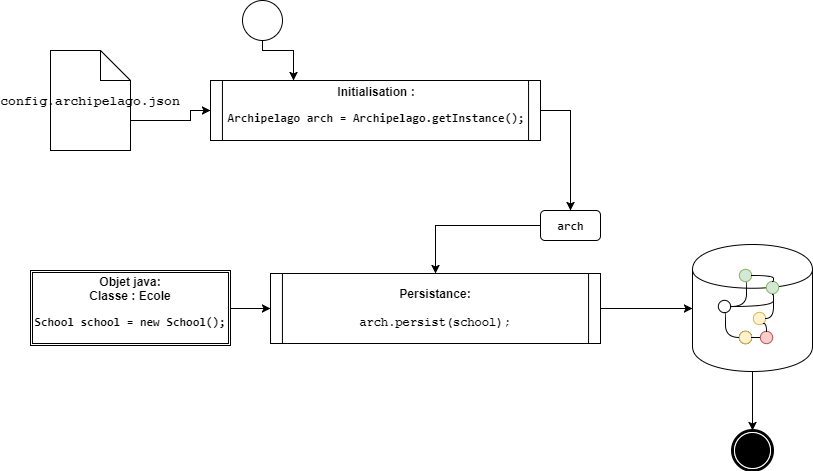
\includegraphics[scale=0.5]{figures/Persist.png}
\label{fig:Persist}
\end{center}
    

\subsection{La récupération}

La récupération de l'information est la raison pour laquelle nous la stockons. A quoi bon enregistrer une valeur dans une base de donnée si nous ne souhaitons jamais l'utiliser ultérieurement ?

Pour cela, Archipelago vient avec un système de création de requête. Grâce à ce procédé, que votre BDOG soit OrientDB ou Neo4J, vous serez en mesure de récupérer votre objet sans changer votre code source. 

Voici un exemple:

\begin{lstlisting}
Archipelago arch = Archipelago.getInstance();

ArchipelagoQuery aq = a.getQueryBuilder()
                .of(Student.class)
                .build();
List<Object> nodes = arch.execute(aq);
\end{lstlisting}

Cette requête va rechercher l'ensemble des étudiants de la base de donnée ainsi que les objets qui leurs sont liés.

Un système de condition est également mit en place, il permet d'affiner le résultat obtenu: 

\begin{lstlisting}
Archipelago arch = Archipelago.getInstance();

ArchipelagoQuery aq = a.getQueryBuilder()
                .of(Student.class)
                .where(of("firstName","Gilles"), ConditionQualifier.Equal)
                .build();
List<Object> nodes = arch.execute(aq);
\end{lstlisting}

Cette requête va quant à elle rechercher les étudiants ayant "Gilles" comme prénom.

Nous pouvons aussi ajouter des opérateurs logique "OU" et "ET" comme suit :
\begin{lstlisting}
Archipelago arch = Archipelago.getInstance();

ArchipelagoQuery aq = a.getQueryBuilder()
                .of(Student.class)
                .where(of("lastName", "Bodart"), ConditionQualifier.EQUAL)
                .and(of("firstName", "Gilles"), ConditionQualifier.EQUAL)
                .or(of("firstName", "Thomas"), ConditionQualifier.EQUAL)
                .build();
List<Object> nodes = arch.execute(aq);
\end{lstlisting}

Le procédé mit en place à l'heure actuel ne permet pas de faire des conditions fortement complexes, il va ajouter l'élément de condition à la suite de la requête actuelle, pour l'exemple précédent, nous aurons donc : 

\begin{lstlisting}[language=SQL]
lastName = "Bodart" AND ( firstName = "Gilles" OR firstName = "Thomas")
\end{lstlisting}

ce qui se retournera donc la liste des étudiants ayant "Bodart" comme nom de famille et "Gilles" ou "Thomas" comme prénom. \`A L'heure actuelle, il n'est cependant pas possible d'effectuer des requêtes sur les relations entre les objets, cette piste est primordiale pour une deuxième version de ce framework.

\begin{center}
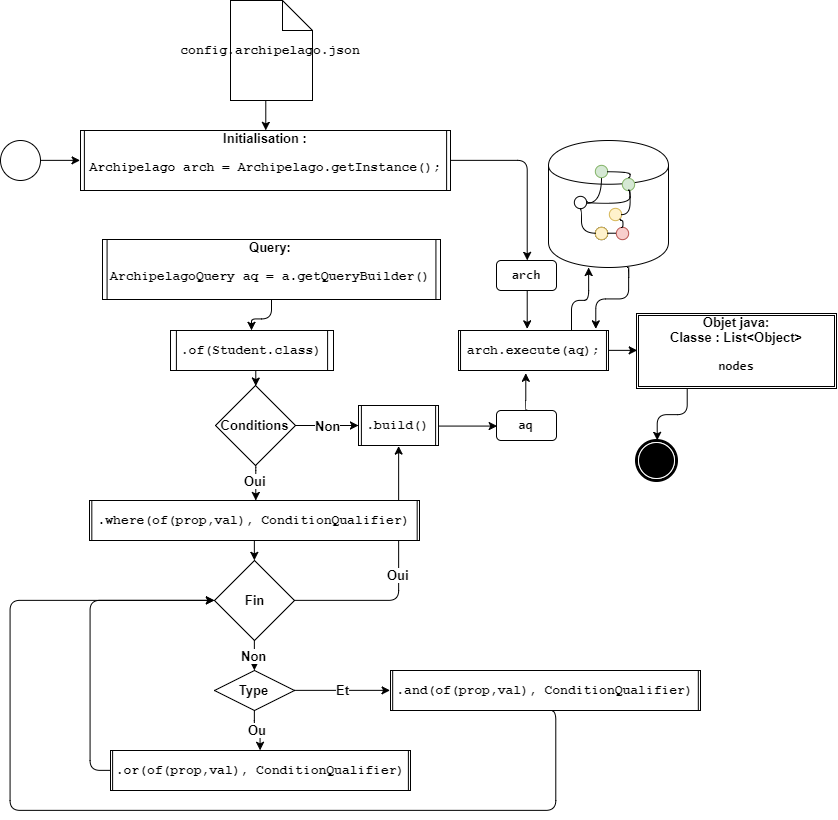
\includegraphics[scale=0.4]{figures/query.png}
\label{fig:Query}
\end{center}

\section{Schema conceptuel}
Les schémas conceptuels représentant une modèle exemple annoté des éléments du framework sera fourni et commenté dans cette section. Cela permettra au lecteur une meilleur compréhension.
\section{Documentation}
Une documentation claire et précise sur l'utilisation du framework Archipelago sera présente dans cette section. Un ensemble entre une documentation fonctionnelle et une documentation technique faite avec JavaDoc.
\section{Processus}
Description du processus implémenté sur base d'un exemple claire. Explications des différents choix d'implémentations et de chaque étape.
\chapter{Evaluation}
\section{Points forts}
Autocritique du framework, sur base de test qualitatif et ou quantitatif. Evaluations : usability, performence, qualité, cohérence
\section{Points faibles}
Autocritique du framework, sur base de test qualitatif et ou quantitatif.
Evaluations : usability, performence, qualité, cohérence
\section{Retour d'information}
Si le temps nous le permet, une analyse des retours utilisateur sera faite en fin de mémoire.
\chapter{Conclusion}
\section{Piste de réflexions}
Une introspection sur le projet sera expliqué dans cette section, les idées innachevés y seront décrites en tant que piste de réflexions.
\section{Archipelago en résumé}
Le mémoire sera conclu avec un explication transversale et complète du framework, permettant au lecteur de garder une bonne impression sur le nouvel outil que sera ce framework.
\part{Annexes}
\begin{sidewaysfigure}[ht]
    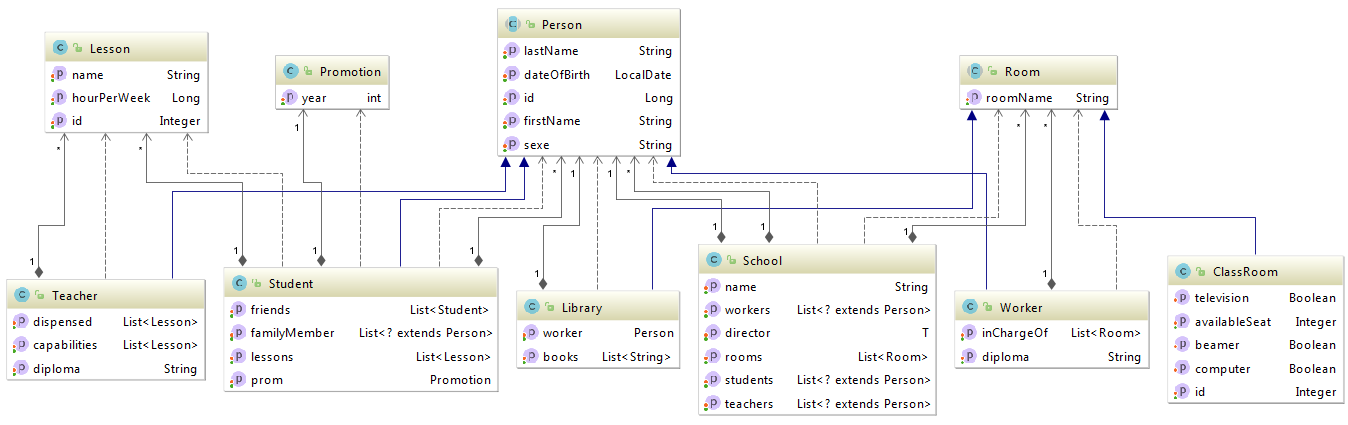
\includegraphics[scale=0.8]{figures/SchoolDiag.png}
    \caption{Diagramme de Classe du modèle École}
    \label{fig:SchoolDiagram}
\end{sidewaysfigure}
\chapter*{Lexique}
\begin{center}
\begin{tabular}[c]{ l p{14cm} }
 SQL  & Structured Query Language \\ \hline
 NoSQL  & Not only SQL \\ \hline
 SGBD  & Système de gestion de base de données \\ \hline
 SGBDR  & Système de gestion de base de données relationnelles \\ \hline
 BDOG  & Base de donnée orientée graph \\ \hline
 JSON  & JavaScript Object Notation \\ \hline
 Vertex  & Sommet \\ \hline
 Edge  & bord \\ \hline
 Cluster  & littéralement grappe, cela représente en informatique un groupe d'élément \\ \hline
 API  & Application Programming Interface  \\ \hline
 REST  & Representational state transfer, style d'architecture pour les systèmes hypermédia distribués \\ \hline
\end{tabular}
\end{center}

\chapter*{Code Sources}
\textbf{ArchipelagoConfig.java}
\lstinputlisting{./src/main/java/org/archipelago/core/configurator/ArchipelagoConfig.java}
\chapter*{Bibliographie}
\begin{itemize}
\item https://neo4j.com/ consulté à de nombreuses reprises (Neo Technology, Inc)
\item https://orientdb.com/ consulté à de nombreuses reprises (OrientDB LTD)
\item https://snap.stanford.edu/data/
\item https://networkx.github.io/
\item http://igraph.org/redirect.html
\item https://snap.stanford.edu/data/egonets-Facebook.html
\item http://konect.uni-koblenz.de/
\item https://icon.colorado.edu/\#!/networks
\item https://neonx.readthedocs.io/en/latest/
\item J. McAuley and J. Leskovec. Learning to Discover Social Circles in Ego Networks. NIPS, 2012.
\item J. Leskovec, K. Lang, A. Dasgupta, M. Mahoney. Community Structure in Large Networks: Natural Cluster Sizes and the Absence of Large Well-Defined Clusters. Internet Mathematics 6(1) 29--123, 2009.
\item https://www.infoq.com/fr/articles/graph-nosql-neo4j
\item http://www.silicon.fr/base-donnees-nosql-impose-sgbdr-93305.html
\item https://prezi.com/4flswlgipwbo/nosql-not-only-sql/
\item [LIVRE] http://www.eyrolles.com/Chapitres/9782212141559/9782212141559.pdf
\item https://db-engines.com
\item https://www.udemy.com/orientdb-getting-started
\item https://fr.wikipedia.org/wiki/Representational\_state\_transfer
\end{itemize}
\end{document}
